\documentclass[leqno, 12pt]{amsart}


%Présentation/langue
\usepackage[english]{babel}
\usepackage[utf8]{inputenc}
\usepackage{geometry}   

\geometry{hmargin=2cm,vmargin=2cm}
\usepackage{lineno}

\usepackage{amsmath}
\usepackage{amssymb}
\usepackage{amsthm}
\usepackage{mathtools}

\numberwithin{equation}{section}

\usepackage{graphicx}
\usepackage{subfig}
\usepackage{caption}
\usepackage{hyperref}
\usepackage{float}
\usepackage{booktabs}
\usepackage[table]{xcolor}

\usepackage{tabularx}

\newcommand{\N}{\mathbb N}
\newcommand{\Z}{\mathbb Z}
\newcommand{\Q}{\mathbb Q}
\newcommand{\R}{\mathbb R}
\newcommand{\K}{\mathbb K}
\newcommand{\Ss}{\mathfrak S}
\newcommand{\Tam}{\mathbf{Tam}}
\newcommand{\dps}{\displaystyle}
\newcommand{\Pos}{\mathcal P}
\renewcommand{\L}{\mathbf L}
\newcommand{\IdL}{\mathbf{Low}}
\newcommand{\IdU}{\mathbf{Upp}}
\newcommand{\JIrr}{\mathcal J}
\newcommand{\MIrr}{\mathcal M}
\newcommand{\Spine}{\mathbf{Spine}}
\newcommand{\Cong}{\mathbf{Cong}}

\newcommand{\pop}{\operatorname{pop}}
\newcommand{\popdown}{\operatorname{pop}^\downarrow}
\newcommand{\popup}{\operatorname{pop}^\uparrow}
\newcommand{\Lmin}{\mathbf 0}
\newcommand{\Lmax}{\mathbf 1}
\newcommand{\JIrrGraph}{\operatorname{JG}}

\newcommand{\Fac}{\mathbf{FInt}}
\newcommand{\SkFac}{\mathbf{FTrv}}
\newcommand{\Int}{\mathbf{Int}}
\newcommand{\SkInt}{\mathbf{Trv}}


\newcommand{\FacGraph}{\operatorname{FInt}}
\newcommand{\SkFacGraph}{\operatorname{FTrv}}
\newcommand{\IntGraph}{\operatorname{Int}}
\newcommand{\SkIntGraph}{\operatorname{Trv}}

%Tamari
\newcommand{\MN}{\operatorname{MN}}
\newcommand{\cvxtopo}{\mathbf{T_{cvx}}}
\newcommand{\treeup}{\mathrm{T_{up}}}
\newcommand{\treedown}{\mathrm{T_{down}}}

%Weak order
\newcommand{\AD}{\operatorname{AscDes}}
\newcommand{\Dec}{\operatorname{Dec}}

\newcommand{\Pairs}{\operatorname{Pairs}}
\newcommand{\inj}{\xhookrightarrow{}}
\newcommand{\surj}{\twoheadrightarrow}

 \DeclareFontFamily{U}{wncy}{}
 \DeclareFontShape{U}{wncy}{m}{n}{<->wncyr10}{}
 \DeclareSymbolFont{mcy}{U}{wncy}{m}{n}
 \DeclareMathSymbol{\Sha}{\mathord}{mcy}{"58} 
 
 \newcommand{\forcingorder}{\mathcal F}
 
 \definecolor{darkblue}{rgb}{0,0,0.7} % darkblue color
 \newcommand{\darkblue}{\color{darkblue}} % darkblue command
 \newcommand{\defn}[1]{\textsl{\darkblue #1}} % emphasis of a definition


\numberwithin{equation}{section}
\newtheorem{thm}{Theorem}[section]
\newtheorem{lem}[thm]{Lemma}
\newtheorem{prop}[thm]{Proposition}
\newtheorem{nota}[thm]{Notation}
\newtheorem{cor}[thm]{Corollary}
\newtheorem{defi}[thm]{Definition}
\newtheorem{cnj}[thm]{Conjecture}
\newtheorem{exmp}[thm]{Example}
\theoremstyle{remark}
\newtheorem{rmk}[thm]{Remark}

\title{Transvals in semidistributive lattices}
\author{Ludovic Schwob}

\begin{document}
	
	\begin{abstract}
	We define transvals, which are a generalization of intervals in semidistributive lattices.
	We show that transvals of the Tamari lattice $\Tam_n$ are in bijection with convex topologies on $\{1,...,n\}$, and that transvals of the weak order on a Weyl group $W$ are in bijection with homogeneous right coideal subalgebras of its quantized enveloping algebra $U_q(\mathfrak g)$.
	\end{abstract}
	
	\maketitle
	
	\tableofcontents
	\section{Introduction}
	
Citer \cite{Hans24} \cite{ClRi15} \cite{BGPPST26} \cite{CPP19} \cite{HeKo12} 
		
\section{Notations and preliminaries}
\subsection{Nuclear intervals (faces)}


%Let $\L$ be a lattice. 
%
%For all $x\in \L$, we define $$x_*:=\begin{cases}
%x \text{ if $x=0$},\\
%\bigwedge_{y\lessdot x}y \text{ otherwise.}
%\end{cases}$$
%
%and $$x^*:=\begin{cases}
%x \text{ if $x=1$},\\
%\bigvee_{x\lessdot y}y \text{ otherwise.}
%\end{cases}$$
%
%In particular, $x_*$ (resp. $x^*$) is the only element covered by $x$ (resp. covering $x$) if $x$ is join-irreducible (resp. meet-irreducible).

   $\L$ be a finite lattice.
  
Let $x\le y\in \L$. We write
    $$\pop_x(y):=y\wedge \bigwedge \{z\in \L: x\le z\lessdot y\}$$
    $$\pop^y(x):=x\vee\bigvee \{z\in \L: x\lessdot z\le y\}.$$

$$\popdown(y):=y\wedge \bigwedge\{x\in \L:x\lessdot y\},$$
$$\popup(x):=x\vee \bigvee\{y\in \L:x\lessdot y\}.$$

When $j$ is a join-irreducible element of $\L$, we also write $j_*:= \popdown(j)$ for the only element covered by $j$. If $m$ is meet-irreducible, we write $m^*:=\popup(m)$.

    Let $[x,y]$ be an interval of $\L$.
    \begin{itemize}
    \item We say that $[x,y]$ is nuclear if $x=\pop_x(y).$
    \item We say that $[x,y]$ is conuclear if $y=\pop^y(x).$
    \item We say that $[x,y]$ is binuclear if it is both nuclear and conuclear.
    \end{itemize}

We also apply the same terminology to finite lattices, by seeing a lattice as its interval $[\Lmin,\Lmax]$.
    
The following assertions are equivalent:
\begin{itemize}
\item $\L$ is meet-semidistributive.
\item The map $\kappa:\JIrr(\L) \to \MIrr(\L)$ sending $j$ to $\kappa(j):=\max\{z:z\wedge j=j_*\}$ is well-defined.
\item Each element of $\L$ has a unique canonical meet-representation.
\end{itemize}
   
	
	\section{Definition of transvals and first results}

\subsection{Faces}

\begin{lem}
   \label{lem:conuclear}
   A finite meet-semidistributive lattice is a nuclear interval if and only if for all atoms $w$ of $\L$, $\kappa(w)$ is a coatom of $\L$.
\end{lem}
\begin{proof}
It is straightforward to check that for all $x\gtrdot\Lmin$, $x=\bigwedge_{y\gtrdot \Lmin , y\neq x}\kappa(y)$ and $\Lmin=\bigwedge_{y\gtrdot \Lmin}\kappa(y)$ (these are the canonical meet-representations of $x$ and $\Lmin$, respectively). Hence, if for all atoms $x$ , $\kappa(x)$ is a coatom, then $\L$ is a nuclear interval. Conversely, if there exists $x\gtrdot \Lmin$ such that $\kappa(x)$ is not a coatom, it implies that for all coatoms $y\lessdot \Lmax$, we have $x\le y$, so their meet is above $x$ and $\L$ is not nuclear.
\end{proof}

\begin{prop}
   Let $\L$ be a finite meet-semidistributive lattice. Let $[x,y]$ be a conuclear interval of $\L$. Then $[x,y]$ is a nuclear interval.
\end{prop}
\begin{proof}
\label{pr:conuclear_implies_nuclear}
   Without loss of generality, we take $\L=[x,y]$. Since $\L$ is conuclear, for all atoms $z\gtrdot x$, there exists $w\lessdot y$ such that $z\nleq w$ (if not, the join of the atoms would be less than $w$), and then $z\wedge w=x$ so $w=\kappa(z)$. By Lemma~\ref{lem:conuclear}, $[x,y]$ is nuclear.
\end{proof}
The converse is not true (see Figure~\ref{fig:inclusionoffaces}).
It follows from Proposition~\ref{pr:conuclear_implies_nuclear}, and from its dual counterpart for join-semidistributive lattices, that in a semidistributive lattice, nuclear and conuclear intervals are the same. We will call \defn{faces} the binuclear intervals of a semidistributive lattice, as they coincide with geometric faces of many polytopal realizations of lattices such as the weak order and the Tamari lattice. However, faces of a semidistributive lattice do not always have a geometric interpretation (see Figure~\ref{fig:inclusionoffaces}).

We have seen in Lemma~\ref{lem:conuclear} that in a nuclear interval $[x,y]$, we have an injection from the atoms to the coatoms of $[x,y]$. In semidistributive lattices this is a bijection. We call the \defn{dimension} of a face $[x,y]$ its number of atoms of this interval, or equivalently its number of coatoms.
 
\begin{figure}[H]
\centering
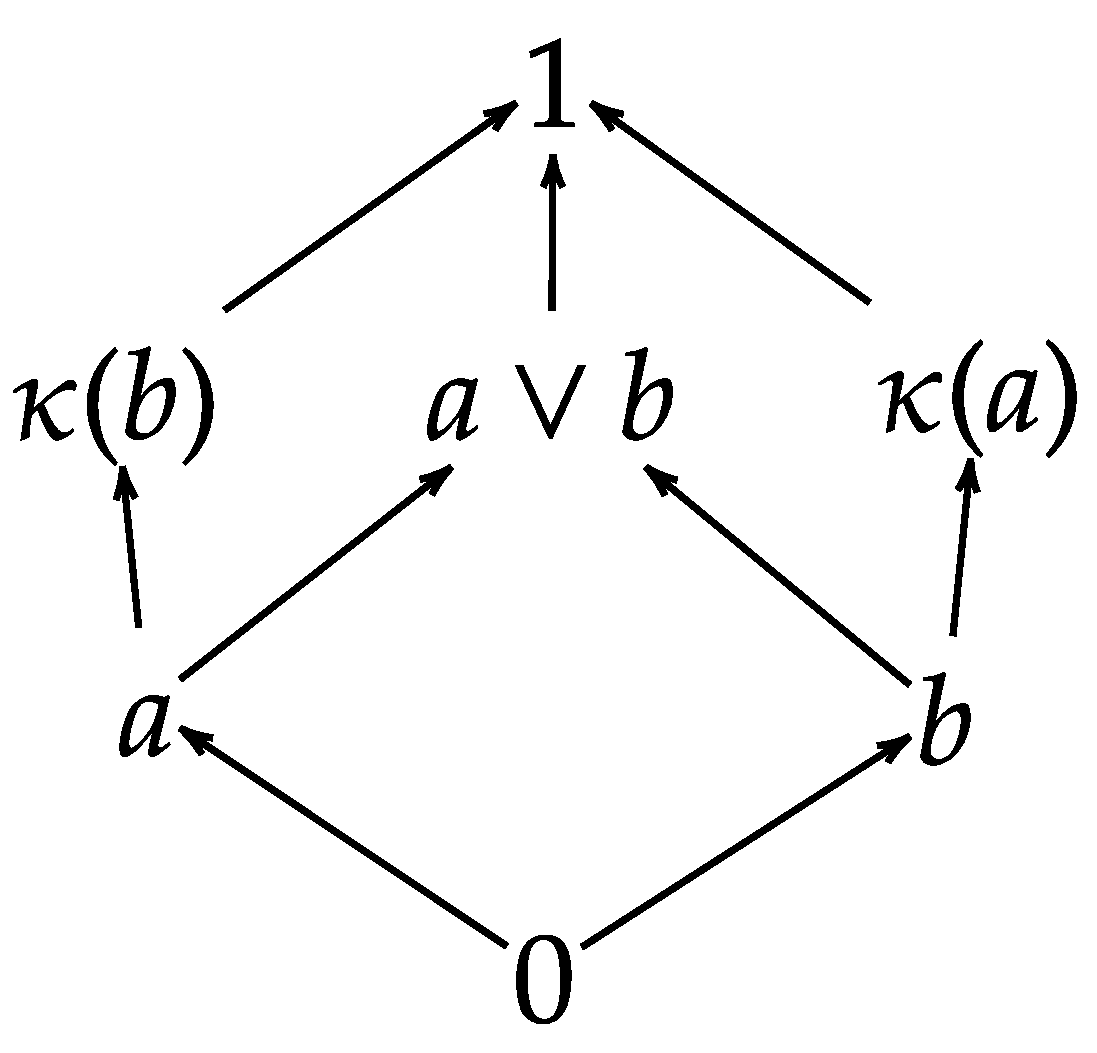
\includegraphics[width=0.4\linewidth]{figures/nuclear_interval}\qquad
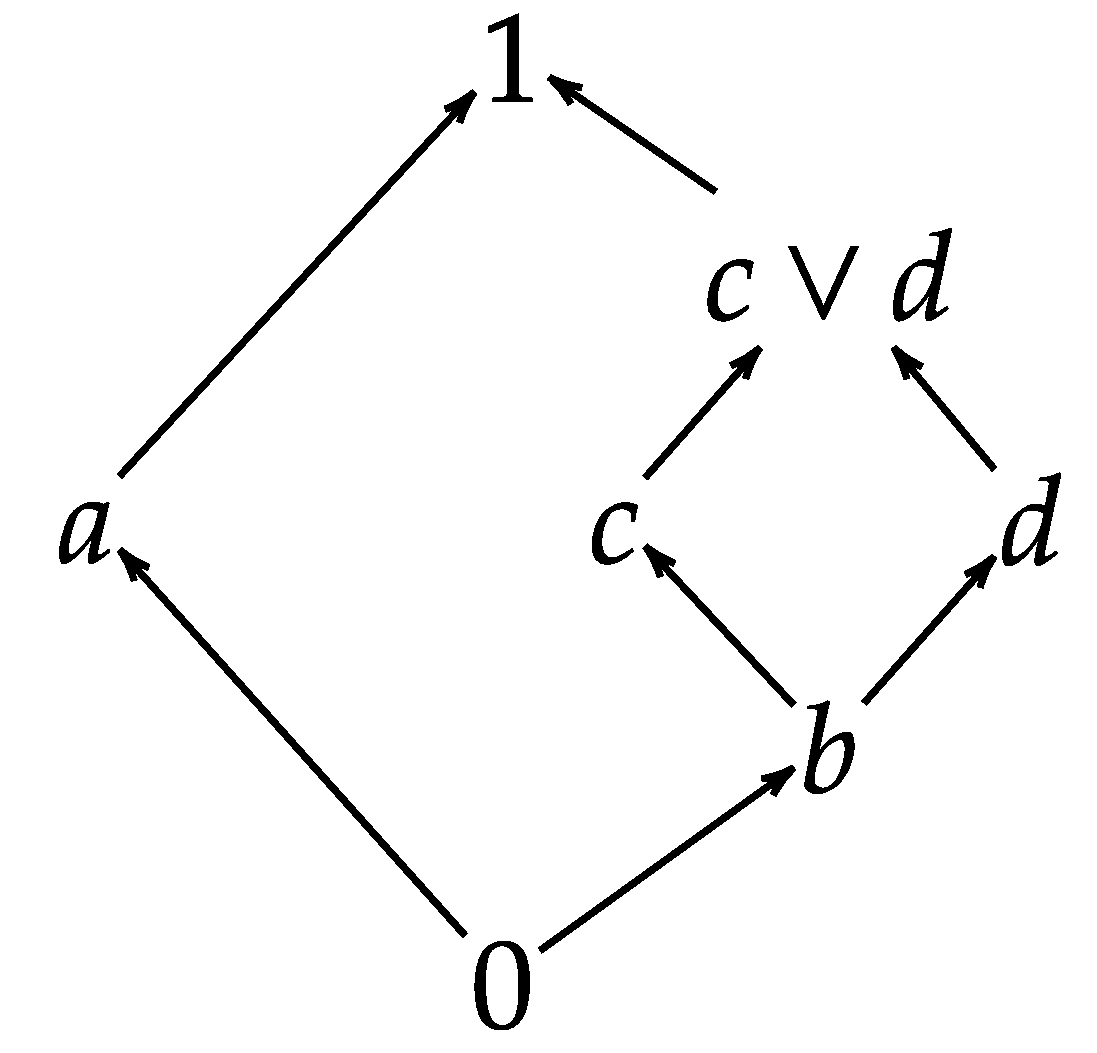
\includegraphics[width=0.4\linewidth]{figures/inclusion_of_faces}
\caption{Left: a meet-semidistributive lattice which is nuclear but not conuclear. Right: A semidistributive lattice with two faces of dimension $2$, one containing the other.}
\label{fig:inclusionoffaces}
\end{figure}


The join of two nuclear intervals is given by $[x_1,y_1]\vee[x_2,y_2]=\left[\popdown_{x_1\vee x_2} (y_1\vee y_2), y_1\vee y_2\right]$. Hanson proved that for any lattice, if its nuclear intervals compared coordinatewise form a lattice then their join has this expression~\cite{Hans24}.
%$$[x_1,y_1]\vee[x_2,y_2]=\left[\bigwedge\{z:x_1\vee x_2\le z\lessdot y_1\vee y_2\}\cup \{y_1\vee y_2\}, y_1\vee y_2\right]$$
	
	\subsection{Transvals}
	
	\begin{defi}
	    Let $\L$ be a lattice, and $x,y\in \L$. The pair $(x,y)$ is a transval of $\L$ if $x_*\le y$ and $x\le y^*$.
	\end{defi}
	
	In the following, $\L$ is a finite semidistributive lattice.
	
	\begin{defi}
		$K_\L$ is the set of atoms $a\in \L$ such that $\kappa(a)$ is a coatom of $\L$.
	\end{defi}
	\begin{prop}
	Let $\L$ be a finite semidistributive lattice. Transvals of $\L$ are the pairs $\left(\bigvee J, \bigwedge \kappa_{[x,y]}(J)\right)$ where $[x,y]$ is an interval of $\L$ and $J\subset K_{[x,y]}$.
	\end{prop}
	\begin{proof}
	   It is straightforward to show that $\left(\bigvee J\right)_*\le x\le y$ and $\left(\bigwedge \kappa(J)\right)^*\ge y\le x$. Conversely, if $(x,y)$ is a transval of $\L$, for all $z$ such that $x\wedge y\lessdot z \le x$, there exists $w\lessdot x\vee y$ such that $z\nleq w$ (if not, we would have $z \le \bigwedge_{y\le w\lessdot x\vee y}w=y$ and $z\le x\wedge y$). Hence we have $y\le \kappa_{[x\wedge y,x\vee y]}(z)\lessdot x\vee y$. Dually, each coatom of $[x\wedge y,x\vee y]$ which is above $y$ correspond to an atom below $x$, implying that $(x,y)=\left(\bigvee J ,\bigvee \kappa{[x\wedge y,x\vee y]}(J)\right)$ where $J=\{z:x\wedge y\lessdot z\le x\}$ and we have $\kappa{[x\wedge y,x\vee y]}(J)\subset \{w:y\le w\lessdot x\vee y\}$.
	\end{proof}
	
	\begin{cor}
		Transvals of $\L$ are in bijection with triples $(x,y,J)$ where $x\le y\in \L$ and $J\subset K_{[x,y]}$.
		\label{cor:bijection_transvals}
	\end{cor}
	
	\begin{prop}
		Let $[x,y]$ be an interval of $\L$. $(y,x)$ is a transval of $\L$ if and only if $[x,y]$ is a nuclear interval.
	\end{prop}
	
	
	Transvals form a lattice whose join is given by $$(x_1,y_1)\vee (x_2,y_2)=(x_1\vee x_2, ?????)$$
	
\subsection{Face transvals}


\section{Lattice structures of transvals}
\begin{prop}
     $\Fac_\L$ is a sublattice of $\SkFac_\L$, and $\Int_\L$ is a sublattice of $\SkInt_\L$.
\end{prop}
However, $\Fac_\L$ is not a sublattice of $\Int_\L$, and $\SkFac_\L$ is not a sublattice of $\SkInt_\L$.  $\SkFac_\L$ contains another sublattice isomorphic to $\Fac_\L$, consisting of pairs $(x,y)$ such that $[x,y]\in \Fac_\L$.

\begin{prop}
Join-irreducible elements of $\Int_\L$, $\SkInt_\L$, $\Fac_\L$, and $\SkFac_\L$ are respectively the elements of the form:
\begin{itemize}
\item $(0,j)$ and $(j,j)$;
\item $(0,j)$ and $(j,j_*)$;
\item $(j_*,j)$ and $(j,j)$;
\item $(j_*,j)$ and $(j,j_*)$;
\end{itemize}
where $0$ is the minimal element of $\L$, and $j\in \JIrr(\L)$.

Meet-irreducible elements of $\Int_\L$, $\SkInt_\L$, $\Fac_\L$, and $\SkFac_\L$ are respectively:
\begin{itemize}
\item $(m,1)$ and $(m,m)$;
\item $(m,1)$ and $(m^*,m)$;
\item $(m,m^*)$ and $(m,m)$;
\item $(m,m^*)$ and $(m^*,m)$;
\end{itemize}
where $1$ is the maximal element of $\L$, and $m\in \MIrr(\L)$.
\end{prop}

\begin{prop}
   The $\kappa$ maps of $\Int_\L$, $\SkInt_\L$, $\Fac_\L$, and $\SkFac_\L$ are respectively given by:
	\begin{itemize}
	\item $(0,j)\mapsto (m,m)$ and $(j,j)\mapsto (m,1)$;
	\item $(0,j)\mapsto(m^*, m)$ and $(j,j_*)\mapsto(m, 1)$;
	\item $(j_*,j\mapsto(m, m)$ and $(j,j)\mapsto(m, m^*)$;
	\item $(j_*,j)\mapsto(m^*, m)$ and $(j,j_*)\mapsto(m , m^*)$;
	\end{itemize}
	where $m=\kappa(j)$.
\end{prop}

\subsection{Cover relations}

Cover relations of $\Fac_\L$ are also of the form $(x,y_1)\lessdot (x,y_2)$ or $(x_1,y)\lessdot (x_2,y)$.

Cover relations of $\SkInt_\L$ are also of the form $(x,y_1)\lessdot (x,y_2)$ or $(x_1,y)\lessdot (x_2,y)$. This comes from the fact that for all $(a,b)\le (c,d)\in \SkInt_\L$, we have $a_*\le b\le d$ and $a\le c\le d^*$, hence $(a,d)$ is a transval of $\L$ with $(a,b)\le (a,d)\le (c,d)$.

However, cover relations of $\SkFac_\L$ are not always of this form (there is a counterexample for $\Tam_3$).
\subsection{Irreducibles graph}

Let $(\Sha, \rightarrow)$ be the two-acyclic factorization system such that $\L \cong \Pairs(\rightarrow)$.

\begin{defi}
  $\IntGraph(\Sha)$,  $\FacGraph(\Sha)$,  $\SkIntGraph(\Sha)$ and  $\SkFacGraph(\Sha)$ are the sets of pairs $(x,k)$ with $x\in \Sha$ and $k\in \{0,1\}$, endowed with respective binary relations
  \begin{itemize}
  \item $(x,0)\rightarrow_{\IntGraph} (x,0)$ and $x\rightarrow y$ implies $(x,k)\rightarrow_{\IntGraph} (y,k)$ for $k\in \{0,1\}$ and $(x,0)\rightarrow_{\IntGraph} (y,1)$;
  \item $x\rightarrow y$ implies $(x,k)\rightarrow_{\SkIntGraph} (y,k)$ for $k\in \{0,1\}$ and $(x,0)\rightarrow_{\SkIntGraph} (y,1)$;
  \item $(x,0)\rightarrow_{\FacGraph} (x,0)$ and $x\rightarrow y$ implies $(x,k)\rightarrow_{\FacGraph} (y,k)$ for $k\in \{0,1\}$, $(x,0)\rightarrow_{\FacGraph} (y,1)$, and $(x,1)\rightarrow_{\FacGraph} (y,0)$;
   \item $x\rightarrow y$ implies $(x,k)\rightarrow_{\SkFacGraph} (y,k)$ for $k\in \{0,1\}$, $(x,0)\rightarrow_{\SkFacGraph} (y,1)$, and $(x,1)\rightarrow_{\SkFacGraph} (y,0)$.
  \end{itemize} 
\end{defi}


\begin{prop} We have the following isomorphisms:
\begin{itemize}
   \item $\Int_\L\cong \Pairs(\rightarrow_{\IntGraph})$.
   \item $\Fac_\L\cong \Pairs(\rightarrow_{\FacGraph})$.
   \item $\SkInt_\L\cong \Pairs(\rightarrow_{\SkIntGraph})$.
   \item $\SkFac_\L\cong \Pairs(\rightarrow_{\SkFacGraph})$.
\end{itemize}
\end{prop}

\subsection{Spine of the lattice transvals in extremal lattices}

Let $\L$ a finite semidistributive lattice. $\L$ is trim if and only if it is extremal~\cite[Thm. 1.4]{ThWi19}. The spine of a trim lattice is its subposet $\Spine(\L)$ formed by elements belonging to a maximal chain. It is a distributive lattice with the same height as $\L$, hence it has the same number of irreducible elements.

\begin{prop}Let $\L$ be a finite semidistributive extremal lattice. We have
   \begin{itemize}
   \item $\Spine(\Int_\L)=\Int_{\Spine(\L)}$;
   \item $\Spine(\SkInt_\L)=\SkInt_{\Spine(\L)}$;
   \item $\Spine(\Fac_\L)=\Fac_{\Spine(\L)}$;
   \item $\Spine(\SkFac_\L)=\SkFac_{\Spine(\L)}$.
   \end{itemize}
\end{prop}
\begin{proof}
Direct proof or corollary of the description of TAFS.
\end{proof}

\section{Canonical join-representations}

\begin{defi}
  Let $G$ be a directed graph. A min-max set of $G$ is a subset $X\subset G$ such that for all $x\in X$, there is no $y,z\in X$ such that $y\to x\to z$.
\end{defi}

%interval-closed subsets of a poset $\Pos$ are in bijection with pairs of disjoint antichains $(A,B)$ of $\Pos$ such that $B\subset \Delta(A)$~\cite[Proposition 2.5]{ELMSW24}. 

\begin{defi}
  An independant set of $G$ is a subset $X\subset G$ such that $x\in X$, there is no $y\in X$ such that $x\to y$ or $y\to x$.
\end{defi}

%Let $\L$ be a finite semidistributive lattice, and let $\JIrrGraph(\L)$  be its irreducibles graph. There is a canonical labelling of edges $\gamma : E(\L)\to \JIrr(L)$ such that for all $(x,y)\in E(\L)$, $y = x\vee \gamma((x,y))$.

%{\color{red}
%FFFFAAAAAAAUUUUUUUXXXXX (par ex. $\Tam_4$)
%\begin{prop}
%   Min-max subsets of $\JIrrGraph(\L)$ are in bijection with edge-labellings of intervals, \emph{i.e.}, sets of the form $\{\gamma((a,b)):(a,b)\in E([x,y])\}$ with $x\le y\in \L$. 
%   Independent sets of $\JIrrGraph(\L)$ are in bijection with labellings $\{\gamma((a,b)):(a,b)\in E([x,y])\}$ where $[x,y]$ is a face of $\L$.
%\end{prop}
%\begin{proof}
%    Let $x\le y\in \L$, $m:=\{\gamma((x,a)):x\lessdot a\le y\}$, and $M:=\{\gamma((b,y)):x\le b\lessdot y\}$. The union $m\cup M$ is a min-max subset of $\JIrrGraph(L)$, and it is an independant set if and only if $m=M$, \emph{i.e.}, $[x,y]$ is a face of $\L$. (show that elements of $m\cup M$ that are both minimal and maximal are $m\cap M$). 
%    %TODO find reverse bijection between set of labels and min-max sets
%\end{proof}}


Let $\L$ be a finite semidistributive lattice, with irreducibles graph $\JIrrGraph(\L)$.
\begin{prop}
   There is a bijection between intervals $(x,y)\in \Int_\L$ and triples $(X,m,M)$ where $X$ is a min-max set of $G$, $\min(X)\subset m$, $\max(X)\subset M$, and $m\sqcup M=X$, which is given by : $(x,y)$ has canonical join-representation $$\bigvee_{j\in m} (0,j)\vee \bigvee_{j\in M} (j,j).$$
\end{prop}

\begin{prop}
    There is a bijection between transvals $(x,y)\in \SkInt_\L$ and triples $(X,m,M)$ where $X$ is a min-max set of $G$, $\min(X)\subset m$, $\max(X)\subset M$, and $m\cup M=X$, which is given by : $(x,y)$ has canonical join-representation $$\bigvee_{j\in m} (0,j)\vee \bigvee_{j\in M} (j,j_*).$$
 Intervals of $\L$ correspond to triples $(X,m,M)$ such that $M\subset m=X$.
\end{prop}

\begin{prop}
   There is a bijection between faces $(x,y)\in \Fac_\L$ and triples $(X,m,M)$ where $X$ is an independent set of $G$, $\min(X)\subset m$, $\max(X)\subset M$, and $m\sqcup M=X$, which is given by : $(x,y)$ has canonical join-representation $$\bigvee_{j\in m} (j_*,j)\vee \bigvee_{j\in M} (j,j).$$
\end{prop}

\begin{prop}
  There is a bijection between face transvals $(x,y)\in \SkFac_\L$ and triples $(X,m,M)$ where $X$ is an independent set of $G$, $\min(X)\subset m$, $\max(X)\subset M$, and $m\cup M=X$, which is given by : $(x,y)$ has canonical join-representation $$\bigvee_{j\in m} (j_*,j)\vee \bigvee_{j\in M} (j,j_*).$$
    Faces of $\L$ correspond to triples $(X,m,M)$ such that $M\subset m=X$.
\end{prop}

\subsection{Enumeration of interval-closed subsets}

If $G$ is transitive, its min-max subsets are in bijection with interval-closed subsets of $G$ seen as a poset. In~\cite{ELMSW24}, the authors generalized rowmotion to interval-closed subsets of posets. It would be interesting to generalize this further on min-max subsets of semidistributive lattices. They showed that interval-closed subsets are in bijection with pairs of disjoint antichains $(A,B)$ such that $B\subset \downarrow A$.

We define two different orders on the set of interval-closed subsets of a poset $\Pos$, and we prove that these orders are join-distributive lattices. Join-lattices can be represented by colored posets, generalizing the Birkhoff's representation theorem~\cite{HaNo18}.

The reverse inclusion of interval-closed subsets yields a join-distributive lattice whose corresponding colored poset is $$(\Pos\setminus \max(\Pos))\sqcup \overline{(\Pos\setminus \min(\Pos))},$$
where elements of $\Pos$ which are neither maximal nor minimal give two distinct elements with the same color.

\begin{figure}[H]
\centering
\raisebox{60pt}{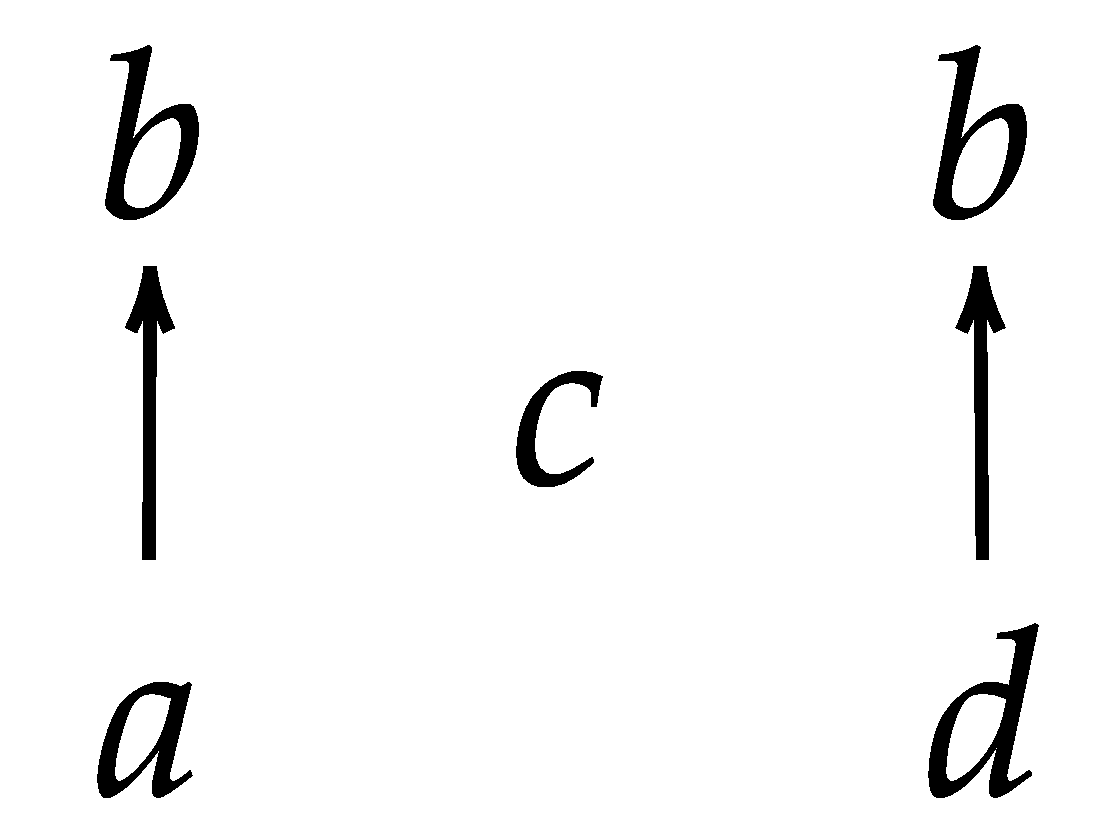
\includegraphics[width=0.2\linewidth]{figures/colored_poset1}}\hspace{60pt}
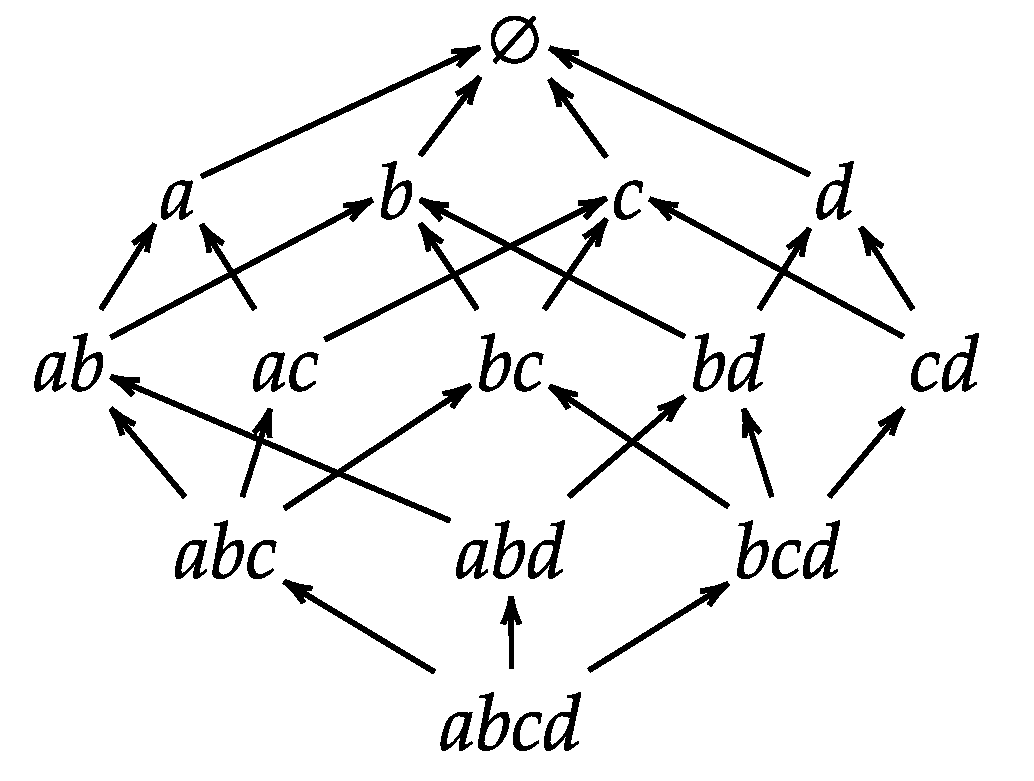
\includegraphics[width=0.5\linewidth]{figures/interval_closed_sets1}
\caption{}
\label{fig:coloredposet1}
\end{figure}


The order $(A_1,B_1)\le (A_2,B_2)\iff \downarrow A_1 \subset \downarrow A_2 \text{ and } \downarrow B_1 \subset \downarrow B_2 $ yields a join-distributive lattice whose corresponding colored poset contains elements and edges of $\Pos$, with cover relations given by $$x\lessdot y\lessdot z\in \Pos\implies \begin{cases}
x\lessdot y \\ y\lessdot (x,y) \\ (x,y) \lessdot (y,z) 
\end{cases}.$$
Two edges have the same color if they have the same lower bound.

\begin{figure}[H]
\centering
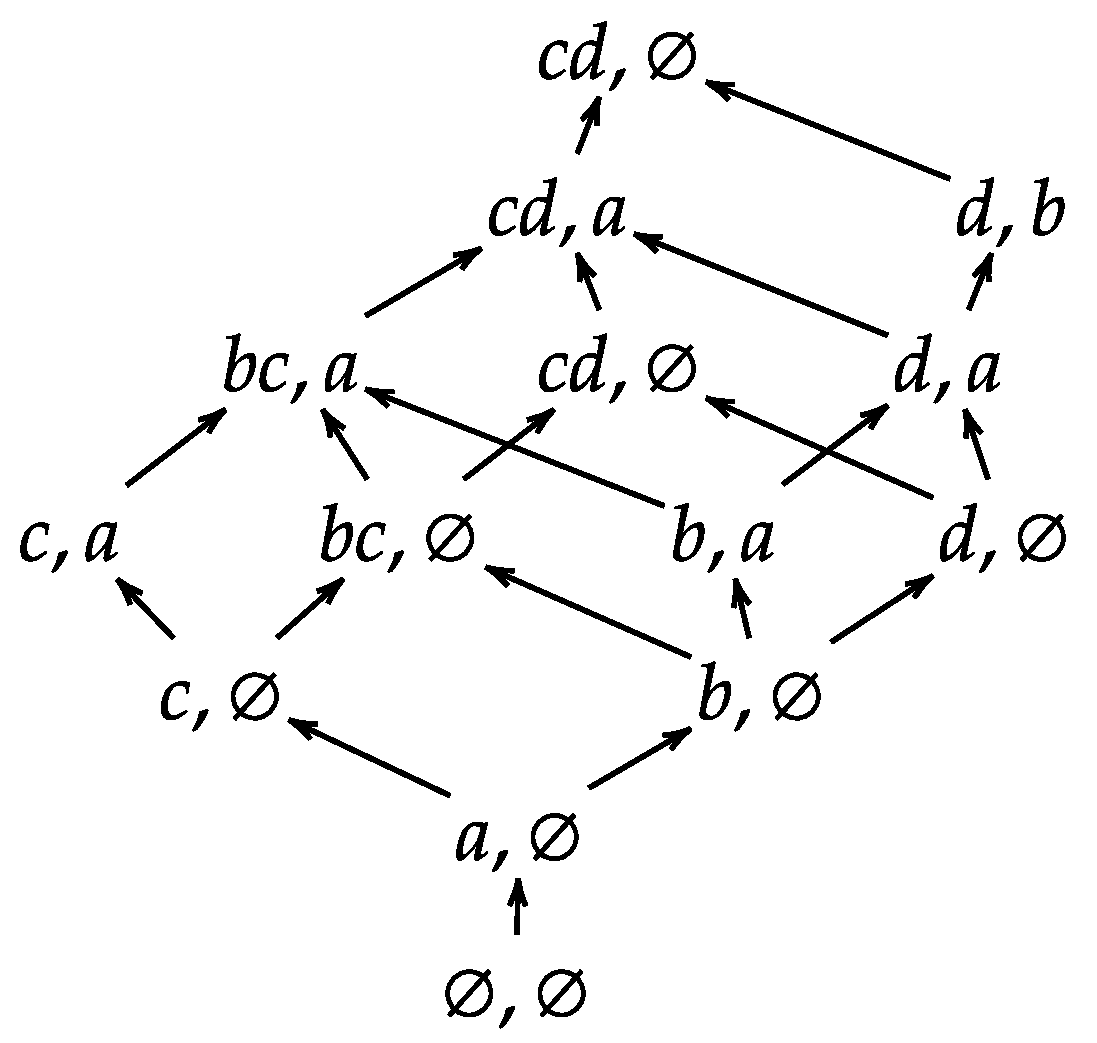
\includegraphics[width=0.5\linewidth]{figures/interval_closed_sets2}
\caption{}
\label{fig:coloredposet2}
\end{figure}

\section{Transvals of the Tamari lattice}
	We show that transvals of the Tamari lattice $\Tam_n$ are in bijection with topologies on $\{1,...,n\}$ having a base of convex sets. These topologies were first enumerated in~\cite{ClRi15}.
	
	Objects equienumerated or in bijection with convex topologies have already been studied in \cite{BGPPST26}, [papier Jonathan Yang ?]
	
	\subsection{Convex topologies}
	
	Let $X$ be a convex topology on $\{1,...,n\}$. Each $k\in \{1,...,n\}$ has a minimal neighborhood in $X$ written $\MN_X(k)$ which is convex by definition. The mapping $k\mapsto \MN_X(k)$ characterizes the topology $X$.
	
	We write $\cvxtopo(n)$ the set of convex topologies on $\{1,\dots, n\}$, with the following order: for all $X,Y\in \cvxtopo(n)$, $X\le Y $ if and only if for all $k\in \{1,...,n\}$, $\MN_X(k) \le \MN_Y(k)$ where minimal neighborhoods are compared coordinatewise.
	Nested convex topologies form a sublattice of convex topologies. The spine of ... has size $A001333(n)$
	
	\begin{figure}[H]
	\centering
	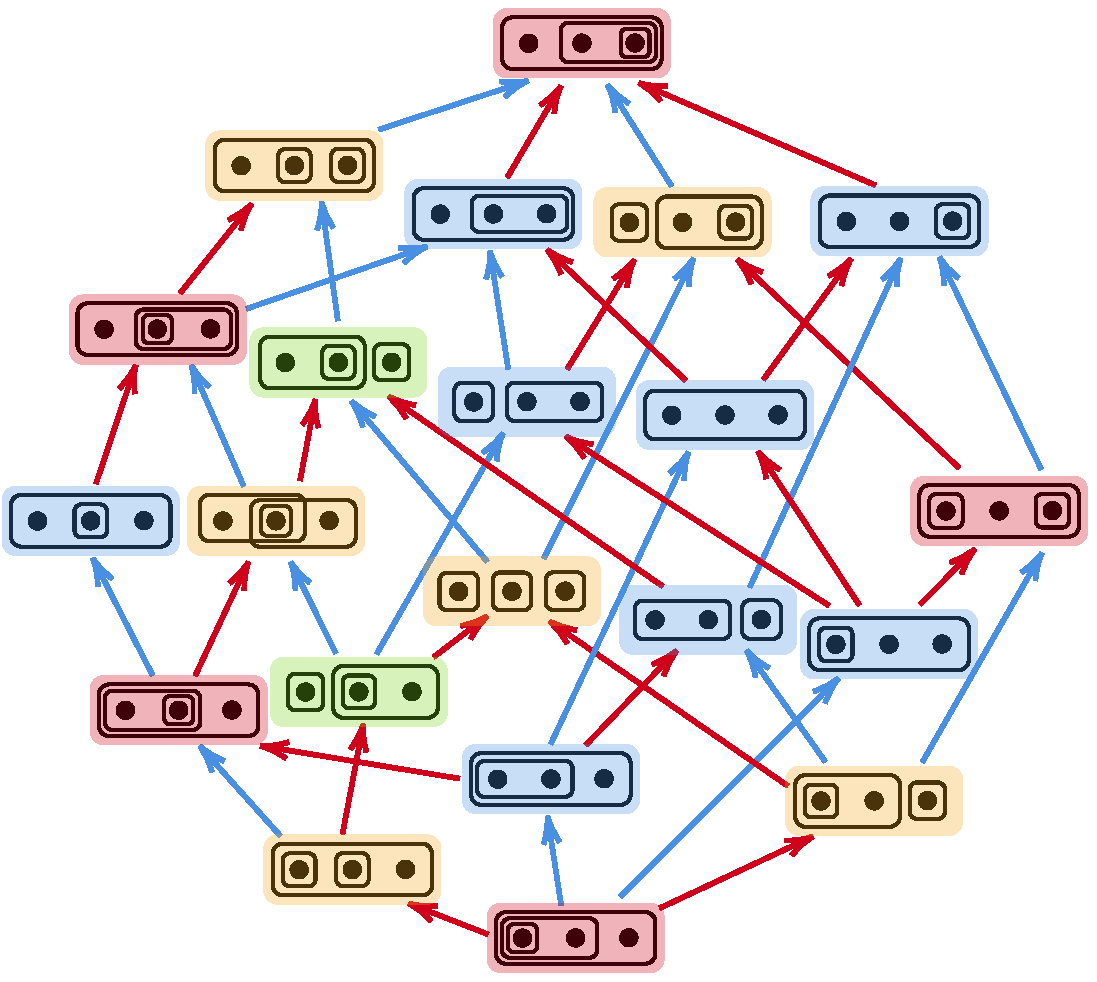
\includegraphics[width=0.7\linewidth]{figures/ConvexTopologies2}
	\caption{The lattice of convex topologies on $\{1,\dots,3\}$.}
	\label{fig:convextopologies}
	\end{figure}
	
We write $\Tam_n$ the Tamari lattice on binary trees of size $n$, \emph{i.e.}, with $n$ internal nodes. 
From a convex topology we construct recursively a binary tree in two different ways.
\begin{defi}
Let $X\in \cvxtopo(n)$. If $X$ is empty, $\treeup(X)$ is the empty binary tree (a leaf). If not, $\treeup(X)$ is the binary tree of size $n$ whose left and right children are respectively $\treeup(X\cap \{1,\dots, k-2\})$ and $\treeup(X\cap \{k,\dots, n\})$ where $2\le k \le n$ is the smallest value such that $\{k,\dots, n\}$ is open in $X$.

If $X$ is empty, $\treedown(X)$ is the empty binary tree. If not, $\treedown(X)$ is the binary tree of size $n$ whose left and right children are respectively $\treedown(X\cap \{1,\dots, k\})$ and $\treedown(X\cap \{k+2,\dots, n\})$ where $1\le k \le 1$ is the biggest value such that $\{1,\dots, k\}$ is open in $X$.
\end{defi}
	
	\begin{prop}
	The map $X\mapsto (\treedown(X),\treeup(X))$ is an isomorphism from $\cvxtopo(n)$ to $\SkInt_{\Tam_n}$.
	\end{prop}
	
	\begin{figure}[H]
	\centering
	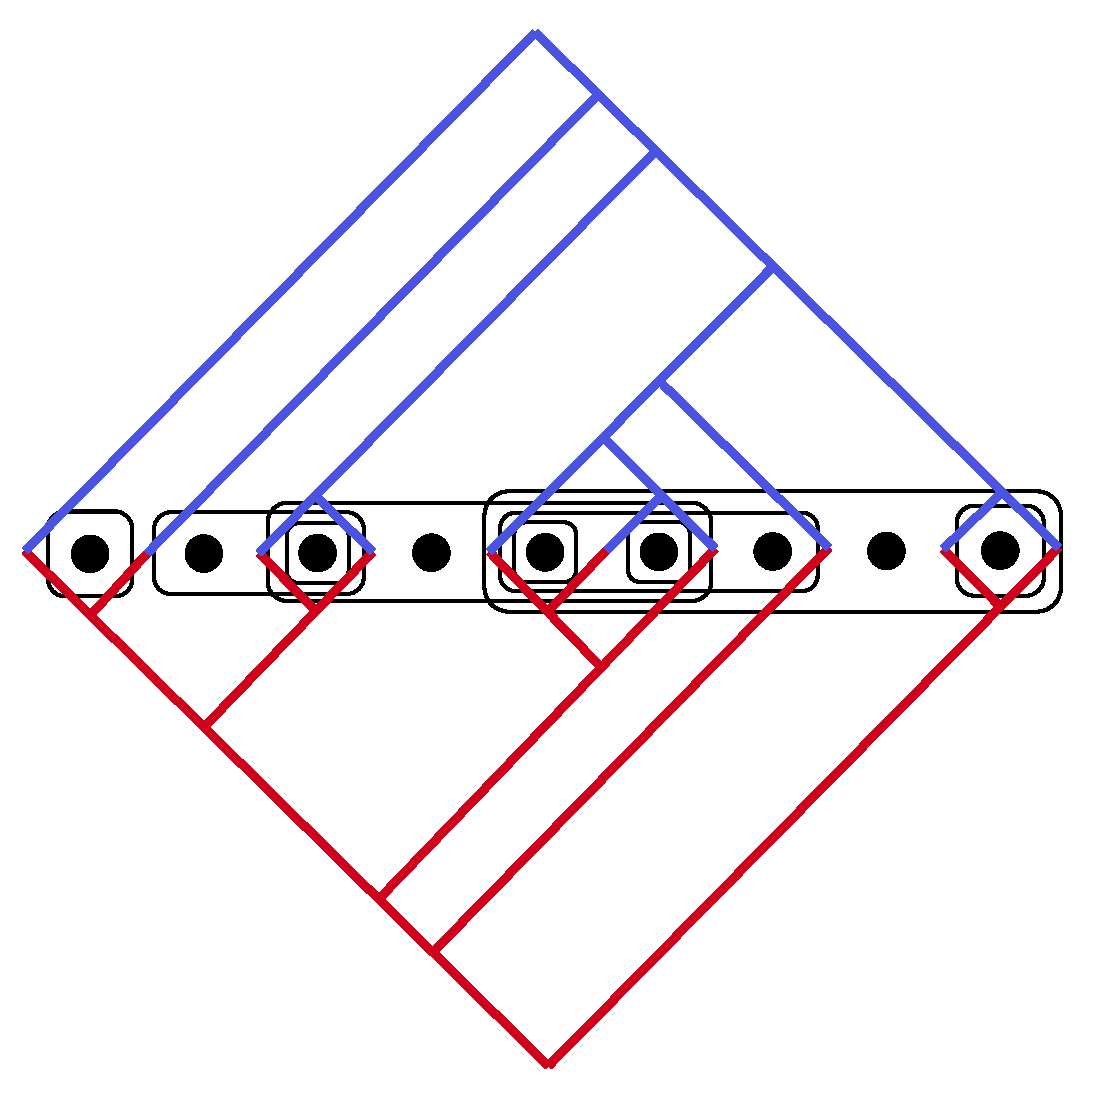
\includegraphics[width=0.45\linewidth]{figures/tamari_transval1} \qquad 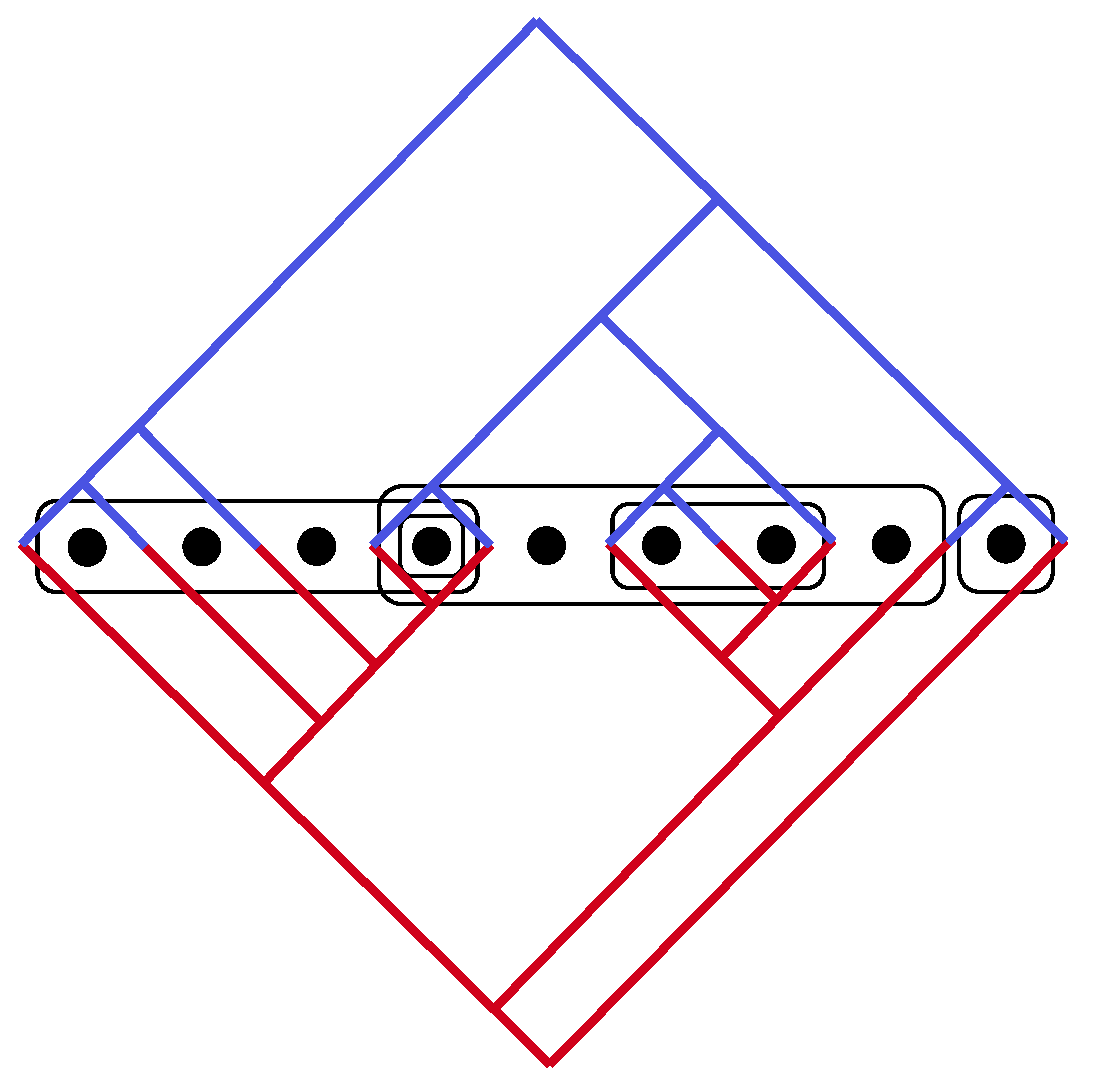
\includegraphics[width=0.45\linewidth]{figures/tamari_transval2}
	\caption{\centering Two transvals of $\Tam_9$ with the corresponding convex topologies. The one on the left is an interval, the one on the right is not.}
	\label{fig:tamaritransval}
	\end{figure}
	
	\begin{prop}
	   Let $X\in \cvxtopo(n)$. $(\treedown(X),\treeup(X))$ is an interval of $\Tam_n$ if and only the minimal neighborhoods $\MN(k)$ are all distinct for $k\in \{1,\dots,n\}$.
	\end{prop}
	
	\begin{table}[H]
		\centering
		\begin{tabular}{ccccccccccc}
		\toprule
		   $n$ & $1$& $2$ &$3$ & $4$ & $5$ & $6$ & $7$ & $8$ & $9$ & $10$  \\ \midrule 
			$A000108$ & $1$ & $2$ & $5$ & $14$ & $42$ & $132$ & $429$ & $1430$ & $4862$ & $16796$  \\ \midrule 
			$A001003$ & $1$ & $3$ & $11$ & $45$ & $197$ & $903$ & $4279$ & $20793$ & $103049$ & $518859$ \\  \midrule
		   $A000260$ & $1$ & $3$ & $13$ & $68$ & $399$ & $2530$ & $16965$ & $118668$ &$857956$ & $6369883$  \\ \midrule 
			$A007564$ & $1$ & $4$ & $19$ & $100$ & $562$ & $3304$ & $20071$ & $124996$ & $793774$ & $5120632$  \\ \midrule 
		    $A234268$ & $1$ & $4$ & $21$ & $129$ & $876$ & $6376$ & $48829$ & $388771$ & $3191849$ & $26864936$  \\  \bottomrule
		\end{tabular}
		\caption{\centering The number of elements, face intervals, intervals, face transvals, and transvals of $\Tam_n$.}
	\end{table}
	
	
	\begin{table}[H]
		\centering
		\begin{tabular}{ccccccccccc}
		\toprule
		   $n$ & $1$& $2$ &$3$ & $4$ & $5$ & $6$ & $7$ & $8$ & $9$ & $10$  \\ \midrule 
		   		 & $1$ & $0$ & $1$ & $0$ & $2$ & $0$ & $5$ & $0$ & $14$ & $0$  \\  \midrule
			 & $1$ & $1$ & $3$ & $3$ & $11$ & $11$ & $45$ & $45$ & $197$ & $197$ \\  \midrule
		   $A369082$ & $1$ & $1$ & $3$ & $4$ & $15$ & $22$ & $91$ & $140$ &$612$ & $969$  \\ \midrule 
			 & $1$ & $2$ & $5$ & $10$ & $28$ & $56$ & $167$ & $334$ & $1036$ &  \\ \midrule 
			& $1$ & $2$ & $5$ & $11$ & $32$ & $74$ & $233$ & $555$ & $1833$ &  \\ \bottomrule

		\end{tabular}
		\caption{\centering The number of self-dual elements, face intervals, intervals, face transvals, and transvals of $\Tam_n$.}
	\end{table}
	
	\subsection{Nested mountains}
	
	
	MENTION TAMARI PREPOSETS ($\to$ SECTION QUOTIENTS OF THE WEAK ORDER),
	
	\subsection{Congruences of the lattice of transvals of $\Tam_n$}
	
	\begin{prop}
		The lattice of congruences of $\SkInt(\Tam_n)$ is isomorphic to the lattice of Motzkin paths of length $2n-1$.
	\end{prop}
	
	\begin{prop}
	     $|\SkFac_{\Tam_n}|=|\Cong(\SkFac_{\Tam_n})|$
	\end{prop}
	
	\begin{table}[H]
		\centering
		\begin{tabular}{ccccccccccc}
		\toprule
		   $n$ & $1$& $2$ &$3$ & $4$ & $5$ & $6$ & $7$ & $8$ & $9$ & $10$  \\ \midrule 
		 $A000108$ & $1$ & $2$ & $5$ & $14$ & $42$ & $132$ & $429$ & $1430$ & $4862$ & $16796$  \\  \midrule 
				$A103211$ & $1$ & $4$ & $28$ & $244$ & $2380$ & $24868$ & $272188$ & $3080596$ & $35758828$ & $423373636$ \\ \midrule
		$A001246$  & $1$ & $4$ & $25$ & $196$ & $1681$ & $2116$ & $18769$ & $168100$ &$1510441$ & $13586596$  \\ \midrule 
		
	    $A007564$ & $1$ & $4$ & $19$ & $100$ & $562$ & $3304$ & $20071$ & $124996$ & $793774$ & $5120632$  \\ \midrule 
        $A099250$	 & $1$ & $4$ & $21$ & $127$ & $835$ & $5798$ & $41835$ & $310572$ & $2356779$ & $18199284$ \\ \bottomrule
		\end{tabular}
		\caption{\centering The number of congruences of the lattices of elements, face intervals, intervals, face transvals, and transvals of $\Tam_n$.}
	\end{table}
	
%	\subsection{Polytopal decompositions}
% pas intéressant, ne semble pas se généraliser aux transvalles
%The lattice of intervals and the lattice of faces decompose into polytopes, whose numbers are :
%	\begin{itemize}
%	\item $\Fac_\L$ : $2^n$
%	\item $\Int_\L$ : nombre d'intervalles synchrones (A000139)
%	\end{itemize}
%

\subsection{The lattice of faces}
	
$\SkInt(\Tam_n)$  contains the lattice of faces of $\Tam_n $ as a subposet of its intervals, {\color{red} FAUX (TAM4) but also as a sublattice containing nested convex topologies (cf. A007052)}
	
\subsection{Transvals of Jurassian lattices}
   Jurassian lattices do not have the same number of transvals or intervals as the Tamari lattice, but it is the case for those obtained from a rectangulation into chains.
	
	\section{Skew intervals of the weak order}
	
	Let $\mathfrak g$ be a finite-dimensional complex semisimple Lie algebra, $W$ its Weyl group, and $U_q(\mathfrak g)$ the quantized enveloping algebra of $\mathfrak g$. Heckenberger and Kolb~\cite{HeKo12} showed that homogeneous right coideal subalgebras of $U_q(\mathfrak g)$ are in bijection with triples $(x,u,J)$ where $x,u\in W$ with $u^{-1}\le_R x$ and $J\subset \Pi\cap x\Pi$, where $\Pi$ denotes a fixed basis of the root system of $\mathfrak g$. We show that they are also in bijection with transvals of the weak order.
	
	
	\begin{defi}
		Let $w\in W$. $(r,s)\in S^2$ is a decoil of $w$ if $wr=sw$ and $l(sw)<l(w)$. We write $\Dec(w)$ the set of decoils of $w$.
	\end{defi}
	\begin{defi}
		Let $u,v \in W$ such that $u\le_Rv$. We define $\AD(u,v)$ as the set containing all $(r,s)\in S^2$ such that $r$ is an ascent of $u$ and $s$ a descent of $v$ corresponding to the same reflection, \emph{i.e.} $u\le_Rur$, $vs\le v$ and $uru^{-1}=vsv^{-1}$.
	\end{defi}
	
	\begin{prop}
		Let $u,v\in W$ such that $u\le_R v$. Elements of $K_{[u,v]}$ are in bijection with elements of $\AD(u,v)$. More precisely, we have $(r,s) \in \AD(u,v)$ if and only if $ur\in K_{[u,v]}$, and in this case $\kappa(ur)=vs$.
		\label{pr:ascents_descents}
	\end{prop}
	\begin{prop}
		Transvals of $(W,\le_R)$  are in bijection with triples $(x,y,K)$ where $x\le_Ry$ and $K$ is a subset of $\Dec(x)$.
	\end{prop}
	\begin{proof}
		By Propositions (\ref{cor:bijection_transvals}) and (\ref{pr:ascents_descents}), transvals of $(W,\le_R)$ are in bijection with triples $(u,v,J)$ where $u\le_R v$ and $J$ is a subset of $\AD(u,v)$. We show that the map $(u,v)\mapsto (v^{-1}u,v^{-1})$ is a bijection between intervals of the right weak order, and that we have $\AD(u,v)=\Dec(v^{-1}u)$ for $u\le_Rv$. We have $u\le_Rv$ if and only $u$ is a prefix of $v$, which is equivalent to $u^{-1}v$ being a suffix of $v$, \emph{i.e.} $u^{-1}v\le_Lv$. By taking inverses, we get $v^{-1}u\le_Rv^{-1}$. Let $(r,s)\in \AD(u,v)$. Since $s$ is a descent of $v$, it is also a descent of $u^{-1}v$ 
	\end{proof}
	
     \begin{table}[H]
			\centering
			\begin{tabular}{ccccccccc}
			\toprule
			   $n$ & $2$ &$3$ & $4$ & $5$ & $6$ & $7$ & $8$ & $9$   \\ \midrule 
				 $A000142$ & $2$ & $6$ & $24$ & $120$ & $720$ & $5040$ & $40320$ & $362880$ \\ \midrule 
				$A000670$ & $3$ & $13$ & $75$ & $541$ & $4683$ & $47293$ & $545835$ & $7087261$   \\ \midrule 
			   $A007767$ & $3$ & $17$ & $151$ & $1899$ & $31711$ & $672697$ & $17551323$ & $549500451$   \\ \midrule 
				 $A122704$ & $4$ & $22$ & $160$ & $1456$ & $15905$ & $202672$ & $2951680$ & $48361216$   \\  \midrule
			    $A213438$ & $4$ & $26$ & $252$ & $3368$ & $58810$ & $1290930$ & $34604844$ & $1107490596$  \\  \bottomrule
			\end{tabular}
			\caption{\centering The number of elements, face intervals, intervals, face transvals, and transvals of $(A_n,\le_R)$.}
		\end{table}
		
     \begin{table}[H]
			\centering
			\begin{tabular}{ccccccc}
			\toprule
			   $n$ & $2$ &$3$ & $4$ & $5$ & $6$ & $7$    \\ \midrule 
			 $A000165$ & $8$ & $48$ & $384$ & $3840$ & $46080$ & $645120$ \\ \midrule 
			 $A080253$ & $17$ & $147$ & $1697$ & $24483$ & $423857$ & $8560947$ \\ \midrule 
			  $A395856$ & $27$ & $457$ & $12069$ & $449439$ & $22145671$ &    \\ \midrule 
			   & $28$ & $304$ & $4432$ &$80704$ & $1763008$ & $44932864$  \\  \midrule
			   $A395854$ & $38$ & $664$ & $17848$ & $672004$ & $33369560$ & $2094849020$  \\  \bottomrule
			\end{tabular}
			\caption{\centering The number of elements, face intervals, intervals, face transvals, and transvals of $(B_n,\le_R)$.}
		\end{table}
		
     \begin{table}[H]
			\centering
			\begin{tabular}{ccccc}
			\toprule
			   $n$ & $4$ & $5$ & $6$ & $7$    \\ \midrule 
			   $A002866$ & $192$ & $1920$ & $23040$ & $322560$\\ \midrule 
			 $A080254$ & $865$ & $12483$ & $216113$ & $4364979$    \\ \midrule 
			  $A395857$ & $3959$ & $146649$ & $7198141$ & $447955715$   \\ \midrule 
			  & $2320$ & $42304$ & $924352$ & $23557888$ \\  \midrule
			   $A395855$ & $6512$ & $238720$ & $11633624$  &  $720453984$  \\  \bottomrule
			\end{tabular}
			\caption{\centering The number of elements, face intervals, intervals, face transvals, and transvals of $(D_n,\le_R)$.}
		\end{table}
		
\section{Transvals of quotients of the weak order}

Bijection between transvals and preposets for any quotient, generalizing \cite{CPP19}

The forcing order of $\Ss_n$ is isomorphic to the poset $\forcingorder_n$ defined as the set of arcs $(a,A,B,b)$ with $1\le a < b\le n$ and $A,B$ a set partition of $\{a+1,\dots, b-1\}$ ($A$ corresponds to points below the arc), ordered by $(a_1,A_1,B_1,b_1) \le (a_2,A_2,B_2,b_2)$ if $a_1\le b_1$, $A_1\subset A_2$, $B_1\subset B_2$ and $b_1\ge b_2$.

\begin{defi}
Let $I\in \IdL(\forcingorder_n)$. A preposet $\blacktriangleleft$ is a weak order quotient preposet if and only if for all $a<b<c$, $a\blacktriangleleft c\implies a\blacktriangleleft b$ or $b\blacktriangleleft c$, and for all $(a,A,B,b)\in I$
\begin{itemize}
\item if $a\blacktriangleleft b$, there exists $k\in A$ such that $a\blacktriangleleft k$, or there exists $k\in B$ such that $k\blacktriangleleft b$;
\item if $a \blacktriangleright b$, there exists $k\in A$ such that $k\blacktriangleright b$, or there exists $k\in B$ such that $a\blacktriangleright k$.
\end{itemize}
\end{defi}
	
	\section{Acknowledgements}
	The numeral coincidences for the number of transvals in the Tamari lattice and the weak order were discovered thanks to the OEIS.
	
\bibliography{Transvals}{}
\bibliographystyle{alpha}
\end{document}